
MEMORIA\\


We have seen in the previous section that
\begin{equation}
\frac{\partial \vec{a}^t}{\partial \vec{a}^k} = \prod_{i=t-1}^{k}  diag(\sigma'(\vec{a}^i)) \cdot \mat{W}^{rec}
\end{equation}

In an equivalent way with can rewtite the previous equation with respect to a couple of neurons $i$ and $j$

\begin{equation}
\frac{\partial \vec{a}_i^t}{\partial \vec{a}_j^k} = \sum_{q\in P(j)} \sum_{l \in P(q)} \hdots \sum_{h : i \in P(h)} w_{qj} \hdots w_{jh} \cdot \sigma'(a_j^k)\sigma'(a_q^{k+1}) \hdots \sigma'(a_i^{t-1})
\label{expanded_mem}
\end{equation}


Observing the previous equation we can argue that each derivatives it's the sum of $p^{t-k-1}$ terms; each term represents the path cost from neuron $i$ to neuron $j$ in the unfolded network, obviously
there are $p^{t-k-1}$ such paths. If we bind the cost $\sigma'(a_l^t)$ to neuron $l$ in the $t^{th}$ layer in the unfolded network we can read the path cost simply surfing the unfolded network multiply
the weight of each arc we walk through and the cost of each neuron we cross, as we can see from figure \ref{gradient_path_cost}.


\tikzstyle{rnn_style}=[->,shorten >=1pt,auto,node distance=1.5cm,
  thick,
  neuron/.style={circle,fill=white!50,draw,minimum size=0.7cm,inner sep=0pt,font=\sffamily\normalsize},
  missing/.style={circle,fill=white!50,draw=none,minimum size=0.7cm,font=\sffamily\Huge\bfseries},
  label/.style={node distance=1.2cm,rectangle,fill=white!50,draw=none,minimum size=0.7cm,font=\sffamily\normalsize},
  thick_edge/.style={line width=1.2pt},
  thin_edge/.style={dotted, line width=0.5pt},
  weight/.style = {above,sloped,pos=0.3},
  ]
\begin{figure}
 \centering
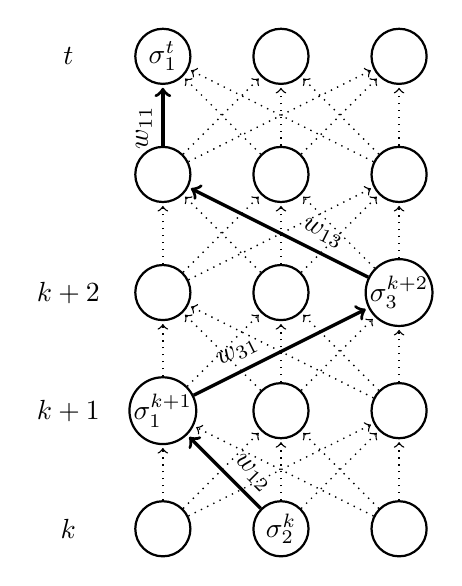
\begin{tikzpicture}[rnn_style]

  
  \node[neuron]    (x1)[]   {$\sigma_1^t$};
  \node[neuron]    (x2)[right of=x1]   {};
  \node[neuron]    (x3)[right of=x2]   {};
  \node[label]     (xl)[left of=x1] {$t$};
  
  \node[neuron]    (h1)[below of =x1]   {$\hdots$};
  \node[neuron]    (h2)[right of=h1]   {};
  \node[neuron]    (h3)[right of=h2]   {};
  \node[label]     (hl)[left of=h1] {$\hdots$};
  
  \node[neuron]    (y1)[below of=h1]   {};
  \node[neuron]    (y2)[right of=y1]   {};
  \node[neuron]    (y3)[right of=y2]   {$\sigma_3^{k+2}$};
  \node[label]     (yl)[left of=y1] {$k+2$};

  
  \node[neuron]    (z1)[below of=y1]   {$\sigma_1^{k+1}$};
  \node[neuron]    (z2)[right of=z1]   {};
  \node[neuron]    (z3)[right of=z2]   {};
  \node[label]     (zl)[left of=z1] {$k+1$};
  
  \node[neuron]    (w1)[below of=z1]   {};
  \node[neuron]    (w2)[right of=w1]   {$\sigma_2^k$};
  \node[neuron]    (w3)[right of=w2]   {};
  \node[label]     (wl)[left of=w1] {$k$};

  
%   \node[label]      (lu)[left of=u] {$u$};
%   \node[label]      (ll)[left of=z1] {$l$};


  \path[->] (h1) edge [thick_edge] node[weight]{$w_{11}$}  (x1)
	    (h1) edge [thin_edge]   (x2)
	    (h1) edge [thin_edge]   (x3)
	    (h2) edge [thin_edge]  (x1)
	    (h2) edge [thin_edge]   (x2)
	    (h2) edge [thin_edge]   (x3)
	    (h3) edge [thin_edge]  (x1)
	    (h3) edge [thin_edge]   (x2)
	    (h3) edge [thin_edge]   (x3);

  \path[->] (y1) edge [thin_edge]   (h1)
	    (y1) edge [thin_edge]   (h2)
	    (y1) edge [thin_edge]   (h3)
	    (y2) edge [thin_edge]   (h1)
	    (y2) edge [thin_edge]   (h2)
	    (y2) edge [thin_edge]   (h3)
	    (y3) edge [thick_edge] node[weight]{$w_{13}$}   (h1)
	    (y3) edge [thin_edge]   (h2)
	    (y3) edge [thin_edge]   (h3);
  
  
  \path[->] (z1) edge [thin_edge]   (y1)
	    (z1) edge [thin_edge]  (y2)
	    (z1) edge [thick_edge] node[weight]{$w_{31}$}   (y3)
	    (z2) edge [thin_edge]  (y1)
	    (z2) edge [thin_edge]  (y2)
	    (z2) edge [thin_edge]  (y3)
	    (z3) edge [thin_edge]   (y1)
	    (z3) edge [thin_edge]   (y2)
	    (z3) edge [thin_edge]   (y3);
	    
  \path[->] (w1) edge [thin_edge]   (z1)
	    (w1) edge [thin_edge]  (z2)
	    (w1) edge [thin_edge]   (z3)
	    (w2) edge [thick_edge] node[weight]{$w_{12}$}   (z1)
	    (w2) edge [thin_edge]   (z2)
	    (w2) edge [thin_edge]   (z3)
	    (w3) edge [thin_edge]   (z1)
	    (w3) edge [thin_edge]   (z2)
	    (w3) edge [thin_edge]   (z3);

	    


\end{tikzpicture}
\caption{The cost for a path from neuron $2$ at time $k$ to neuron $1$ at time $t$ is $w_{12}w_{31}w_{13}\hdots w_{11}\cdot \sigma_2^k \sigma_1^{k+1}\sigma_3^{k+2} \hdots \sigma_1^{t-1} $ }
\label{gradient_path_cost}
\end{figure}


We can further characterize each path cost noticing that we can separate two components, one that depends only on the weights $w_{qj} \hdots w_{jh}$ and the other that depends both on the weights and the inputs
$\sigma'(a_j^k)\sigma'(a_q^{k}) \hdots \sigma'(a_i^{t-1})$.


\paragraph{Hochreiter Analysis: Weak upper bound}

Let's put $$\sigma'_{max} \triangleq \underset{i=k,...,t-1}{\text{max  }} \{||diag(\sigma'(a^i))||_1\}$$.

We have then:
$$\left\Vert \prod_{i=t-1}^{k}  diag(\sigma'(\vec{a}^i)) \cdot \mat{W}^{rec} \right\Vert_1 <= \prod_{i=t-1}^{k} p \cdot ||diag(\sigma'(\vec{a}^i))||_1 \cdot ||\mat{W}^{rec}||_1 $$
since 
$$||diag(\sigma)\cdot \mat{W}||_1 =
\left\Vert 
\begin{array}{c c c c}
\sigma_1 w_{11} & \sigma_1 w_{12} & \hdots & \sigma_1 w_{1p}  \\
\sigma_1 w_{21} & \sigma_2 w_{22} & \hdots & \sigma_2 w_{2p}  \\
\vdots & \vdots  & \vdots & \vdots  \\
\sigma_p w_{p1} & \sigma_p w_{p2} & \hdots & \sigma_p w_{pp}  \\
\end{array}  
\right\Vert_1
<=p \cdot \sigma_{max} \cdot ||\mat{W}||_1
$$

Hence
\begin{align}
\left\Vert \prod_{i=t-1}^{k}  diag(\sigma'(\vec{a}^i)) \cdot \mat{W}^{rec} \right\Vert_1 & <= p \cdot \big(\sigma'_{max}\cdot ||\mat{W}||_1\big)^{t-k-1} \\
& = p \cdot \tau^{t-k-1}
\end{align}
where $$\tau \triangleq \sigma'_{max}\cdot ||\mat{W}||_1$$

So we have exponential decay if $\tau<1$; We can match this condition assuring that
$$\frac{p\cdot ||w_{max}||}{\sigma_{max}}<1$$ where $w_{max}$ is the maxixum value in the weight matrix.


COMPORTAMENTO SBALIATO STRUTTURALE\\
RELU-NON POSSIAMO IMPARARE AD ACCENDERE \\





